\documentclass[a4paper]{article}

\usepackage[czech]{babel} %https://github.com/michal-h21/biblatex-iso690
\usepackage[
   backend=biber      % if we want unicode 
  ,style=iso-numeric % or iso-numeric for numeric citation method          
  ,babel=other        % to support multiple languages in bibliography
  ,sortlocale=cs_CZ   % locale of main language, it is for sorting
  ,bibencoding=UTF8   % this is necessary only if bibliography file is in different encoding than main document
]{biblatex}

\usepackage[utf8]{inputenc}
\usepackage{fancyhdr}
\usepackage{amsmath}
\usepackage{amssymb}
\usepackage[left=2cm,right=2cm,top=2.5cm,bottom=2.5cm]{geometry}
\usepackage{graphicx}
\usepackage{pdfpages}
\usepackage{url}

\usepackage{siunitx}
\sisetup{locale = DE}  %, separate-uncertainty = true    kdybych chtel +/-

\usepackage{float}
\newfloat{graph}{htbp}{grp}
\floatname{graph}{Graf}
\newfloat{tabulka}{htbp}{tbl}
\floatname{tabulka}{Tabulka}

\renewcommand{\thefootnote}{\roman{footnote}}

\pagestyle{fancy}
\lhead{Praktikum I - (IV) Závislost povrchového napětí na koncentraci povrchově aktivní látky}
\rhead{Vladislav Wohlrath}
\author{Vladislav Wohlrath}

\bibliography{source}

\begin{document}

\begin{titlepage}
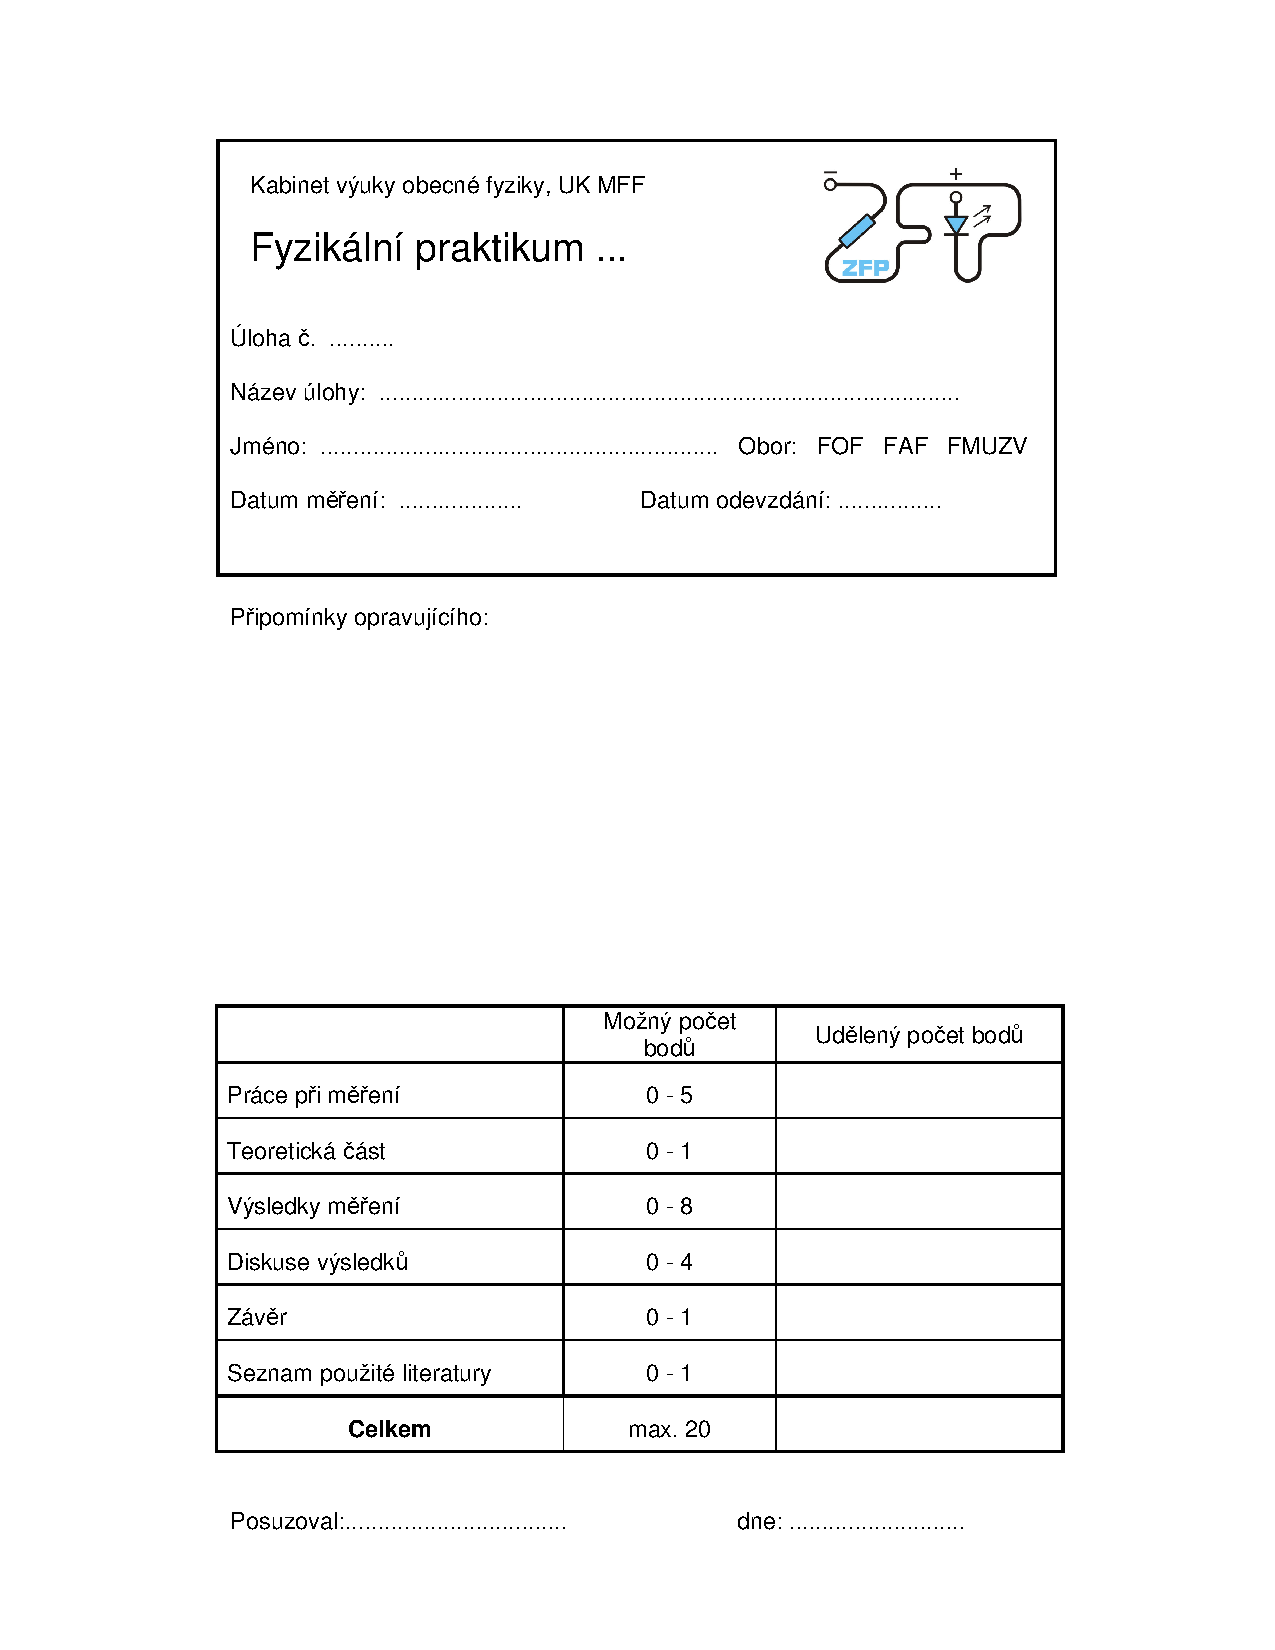
\includepdf[pages={1}]{./graficos/titlelist.pdf}
\end{titlepage}

\section*{Pracovní úkoly}
\begin{enumerate}
\item ÚKOLY \cite{englich} \cite{ZFP}
\end{enumerate}

%Teoretická část
\section*{Teoretická část}
Budeme měřit povrchové napětí roztoku lihu při koncentracích od 0 do \SI{100}{\percent} odtrhávací metodou.
Tato metoda spočívá v měření síly potřebné k odtržení tenkého drátku od hladiny měřené kapaliny.
Pokud je drátek dostatečně tenký a má délku $l$, drží ho kapalina na hladině silou \cite{ZFP}
\begin{equation} \label{eq::p0sigma}
P_0=2 \cdot \sigma \cdot l \,,
\end{equation}
kde $\sigma$ je povrchové napětí.

Sílu $P_0$ budeme měřit torzními vahami.
Na jedno rameno zavěsíme rámeček, ve kterém je upevněn drátek (viz obr. \ref{obr::ramecek}), a pod něj položíme kádinku s měřeným roztokem.
Na druhé rameno pověsíme přívažky tak, aby odtržení drátku od hladiny proběhlo v rozsahu ciferníku torzních vah.

\begin{figure}[htbp]
\centering
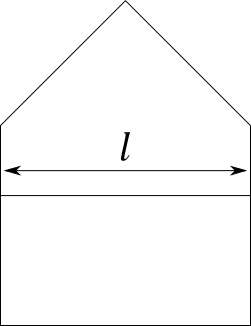
\includegraphics[width=3cm]{graficos/ramecek}
\caption{Náčrt použitého rámečku, na obrázku je vyznačena délka drátku $l$.}
\label{obr::ramecek}
\end{figure}

Protože na drátek nepůsobí pouze síla způsobená povrchovým napětím, změříme nejdříve sílu $P_1$, při které jsou váhy vyvážené a drátek je těsně pod hladinou kapaliny.
Poté budeme sílu zvětšovat a zároveň snižovat kádinku s roztokem, aby váhy zůstali vyvážené.
Při určité síle $P_2$ se drátek odtrhne.
Sílu $P_0$ určíme jako rozdíl sil $P_2$ a $P_1$.

Lenard \cite{oprava} udává korekci na drátek o poloměru $r$
\begin{equation} \label{eq::lenard}
\sigma = \frac{P_0}{2l} - r\left( \sqrt{\frac{P_0 \varrho g}{l}} - \frac{P_0}{l^2} \right) \,,
\end{equation}
kde $\varrho$ je hustota kapaliny a $g$ je tíhové zrychlení.

%Podmínky a měřící přístroje
\section*{Podmínky a použité přístroje}

%Výsledky měření
\section*{Výsledky měření}
Teplota v místnosti byla \SI{23.5(5)}{\degreeCelsius}.
Teplota destilované vody i lihu byla před smícháním stejná.

Drátek v rámečku jsme měřili posuvným měřítkem a měl délku $l = \SI{1.94(5)}{\cm}$.

Na váhy jsme pověsili přívažek o hmotnosti \SI{200}{\milli\g}.
Jelikož síly od sebe odečítáme, nemá přívažek na výsledek žádný vliv.

Torzními vahami jsme přímo měřili rozdíl hmotností na obou ramenech.
Ke změření síly je tedy nutný přepočet na tíhovou sílu $F = mg$, tedy
\begin{equation}
P_1 = m_1 \cdot g \qquad P_2= m_2 \cdot g \,,
\end{equation}
kde $m_1$, $m_2$ jsou váhami změřené rozdíly hmotností na ramenech, když je rámeček těsně pod vodou resp. právě se odtrhl od hladiny, a $g$ je tíhové zrychlení.
Tíhové zrychlení v Praze je \SI{9,814}{\m\per\s\squared} \cite{gravitace}, chybu zanedbáváme.

Vzorec \eqref{eq::p0sigma} má po úpravě a dosazení tvar
\begin{equation}
\sigma = \frac{(m_2-m_1)\cdot g}{2 \cdot l}
\end{equation}

Nejdříve jsme změřili povrchové napětí čisté destilované vody a čistého lihu.
Poté jsme s pomocí pyknometru připravili roztok s \SI{50}{\percent} koncentrací lihu a tento roztok jsme dále ředili vodou vždy v poměru $1:1$.

V tabulce \ref{tab::namereny} jsou pro měřené koncentrace uvedeny hodnoty $m_1$, $m_2$, vypočtené síly $P_0$ a povrchové napětí~$\sigma$.
U $m_1$ a $m_2$ uvádíme přímo číselný údaj na vahách, pro výpočet celkové hodnoty $P_1$ nebo $P_2$ by bylo nutné přičíst hmotnost přívažku.
Směrodatnou odchylku $\mu_m$\footnote{Symbol $\mu$ pro směrodatnou odchylku používáme, aby nedošlo k záměně za povrchové napětí $\sigma$.} určení rozdílu hmotností $(m_2-m_1)$ odhadujeme na \SI{5}{\milli \g}.
Z toho se odvíjí směrodatná odchylka síly $\mu_{P_0} = \SI{0.05}{\milli \newton}$.
Směrodatnou odchylku povrchového napětí počítáme jako
\begin{equation}
\mu_\sigma = \sigma \sqrt{ \left(  \frac{\mu_{P_0}}{P_0} \right)^2 +
\left(  \frac{\mu_{l}}{l} \right)^2   }
\end{equation}

Závislost povrchového napětí na koncentraci lihu v roztoku je zanesena do grafu \ref{grp::graf}.

\begin{tabulka}[htbp]
\centering
\begin{tabular}{ccccc}
koncentrace lihu & $m_1 (\si{\milli\g})$ & $m_2 (\si{\milli\g})$ & $P_0 (\si{\milli \newton})$ & $\sigma (\num{e-3}\,\si{\newton\per\metre})$ \\ \hline 
\SI{0}{\percent} & \num{125} & \num{448} & \num{3.17} & \num{82(3)} \\
\SI{0.4}{\percent} & \num{118} & \num{430} & \num{3.06} & \num{79(3)} \\
\SI{0.8}{\percent} & \num{117} & \num{419} & \num{2.96} & \num{76(3)} \\
\SI{1.6}{\percent} & \num{113} & \num{404} & \num{2.86} & \num{74(3)} \\
\SI{3.1}{\percent} & \num{116} & \num{401} & \num{2.80} & \num{72(3)} \\
\SI{6.3}{\percent} & \num{111} & \num{370} & \num{2.54} & \num{66(3)} \\
\SI{12.5}{\percent} & \num{109} & \num{327} & \num{2.14} & \num{55(2)} \\
\SI{25}{\percent} & \num{106} & \num{277} & \num{1.68} & \num{43(2)} \\
\SI{50}{\percent} & \num{105} & \num{238} & \num{1.31} & \num{34(2)} \\
\SI{100}{\percent} & \num{106} & \num{225} & \num{1.17} & \num{30(2)} \\
\end{tabular}
\caption{Naměřené hodnoty povrchového napětí pro různé koncentrace lihu v roztoku}
\label{tab::namereny}
\end{tabulka}

\begin{graph}[htbp] 
\centering
% GNUPLOT: LaTeX picture with Postscript
\begingroup
  \makeatletter
  \providecommand\color[2][]{%
    \GenericError{(gnuplot) \space\space\space\@spaces}{%
      Package color not loaded in conjunction with
      terminal option `colourtext'%
    }{See the gnuplot documentation for explanation.%
    }{Either use 'blacktext' in gnuplot or load the package
      color.sty in LaTeX.}%
    \renewcommand\color[2][]{}%
  }%
  \providecommand\includegraphics[2][]{%
    \GenericError{(gnuplot) \space\space\space\@spaces}{%
      Package graphicx or graphics not loaded%
    }{See the gnuplot documentation for explanation.%
    }{The gnuplot epslatex terminal needs graphicx.sty or graphics.sty.}%
    \renewcommand\includegraphics[2][]{}%
  }%
  \providecommand\rotatebox[2]{#2}%
  \@ifundefined{ifGPcolor}{%
    \newif\ifGPcolor
    \GPcolorfalse
  }{}%
  \@ifundefined{ifGPblacktext}{%
    \newif\ifGPblacktext
    \GPblacktexttrue
  }{}%
  % define a \g@addto@macro without @ in the name:
  \let\gplgaddtomacro\g@addto@macro
  % define empty templates for all commands taking text:
  \gdef\gplbacktext{}%
  \gdef\gplfronttext{}%
  \makeatother
  \ifGPblacktext
    % no textcolor at all
    \def\colorrgb#1{}%
    \def\colorgray#1{}%
  \else
    % gray or color?
    \ifGPcolor
      \def\colorrgb#1{\color[rgb]{#1}}%
      \def\colorgray#1{\color[gray]{#1}}%
      \expandafter\def\csname LTw\endcsname{\color{white}}%
      \expandafter\def\csname LTb\endcsname{\color{black}}%
      \expandafter\def\csname LTa\endcsname{\color{black}}%
      \expandafter\def\csname LT0\endcsname{\color[rgb]{1,0,0}}%
      \expandafter\def\csname LT1\endcsname{\color[rgb]{0,1,0}}%
      \expandafter\def\csname LT2\endcsname{\color[rgb]{0,0,1}}%
      \expandafter\def\csname LT3\endcsname{\color[rgb]{1,0,1}}%
      \expandafter\def\csname LT4\endcsname{\color[rgb]{0,1,1}}%
      \expandafter\def\csname LT5\endcsname{\color[rgb]{1,1,0}}%
      \expandafter\def\csname LT6\endcsname{\color[rgb]{0,0,0}}%
      \expandafter\def\csname LT7\endcsname{\color[rgb]{1,0.3,0}}%
      \expandafter\def\csname LT8\endcsname{\color[rgb]{0.5,0.5,0.5}}%
    \else
      % gray
      \def\colorrgb#1{\color{black}}%
      \def\colorgray#1{\color[gray]{#1}}%
      \expandafter\def\csname LTw\endcsname{\color{white}}%
      \expandafter\def\csname LTb\endcsname{\color{black}}%
      \expandafter\def\csname LTa\endcsname{\color{black}}%
      \expandafter\def\csname LT0\endcsname{\color{black}}%
      \expandafter\def\csname LT1\endcsname{\color{black}}%
      \expandafter\def\csname LT2\endcsname{\color{black}}%
      \expandafter\def\csname LT3\endcsname{\color{black}}%
      \expandafter\def\csname LT4\endcsname{\color{black}}%
      \expandafter\def\csname LT5\endcsname{\color{black}}%
      \expandafter\def\csname LT6\endcsname{\color{black}}%
      \expandafter\def\csname LT7\endcsname{\color{black}}%
      \expandafter\def\csname LT8\endcsname{\color{black}}%
    \fi
  \fi
  \setlength{\unitlength}{0.0500bp}%
  \begin{picture}(10204.00,6802.00)%
    \gplgaddtomacro\gplbacktext{%
      \csname LTb\endcsname%
      \put(814,704){\makebox(0,0)[r]{\strut{} 20}}%
      \csname LTb\endcsname%
      \put(814,1537){\makebox(0,0)[r]{\strut{} 30}}%
      \csname LTb\endcsname%
      \put(814,2371){\makebox(0,0)[r]{\strut{} 40}}%
      \csname LTb\endcsname%
      \put(814,3204){\makebox(0,0)[r]{\strut{} 50}}%
      \csname LTb\endcsname%
      \put(814,4037){\makebox(0,0)[r]{\strut{} 60}}%
      \csname LTb\endcsname%
      \put(814,4870){\makebox(0,0)[r]{\strut{} 70}}%
      \csname LTb\endcsname%
      \put(814,5704){\makebox(0,0)[r]{\strut{} 80}}%
      \csname LTb\endcsname%
      \put(814,6537){\makebox(0,0)[r]{\strut{} 90}}%
      \csname LTb\endcsname%
      \put(946,484){\makebox(0,0){\strut{} 0}}%
      \csname LTb\endcsname%
      \put(2718,484){\makebox(0,0){\strut{} 20}}%
      \csname LTb\endcsname%
      \put(4490,484){\makebox(0,0){\strut{} 40}}%
      \csname LTb\endcsname%
      \put(6263,484){\makebox(0,0){\strut{} 60}}%
      \csname LTb\endcsname%
      \put(8035,484){\makebox(0,0){\strut{} 80}}%
      \csname LTb\endcsname%
      \put(9807,484){\makebox(0,0){\strut{} 100}}%
      \put(176,3620){\rotatebox{-270}{\makebox(0,0){\strut{}Povrchové napětí (\num{e-3}\,\si{\newton\per\metre})}}}%
      \put(5376,154){\makebox(0,0){\strut{}Koncentrace lihu (\si{\percent})}}%
    }%
    \gplgaddtomacro\gplfronttext{%
    }%
    \gplbacktext
    \put(0,0){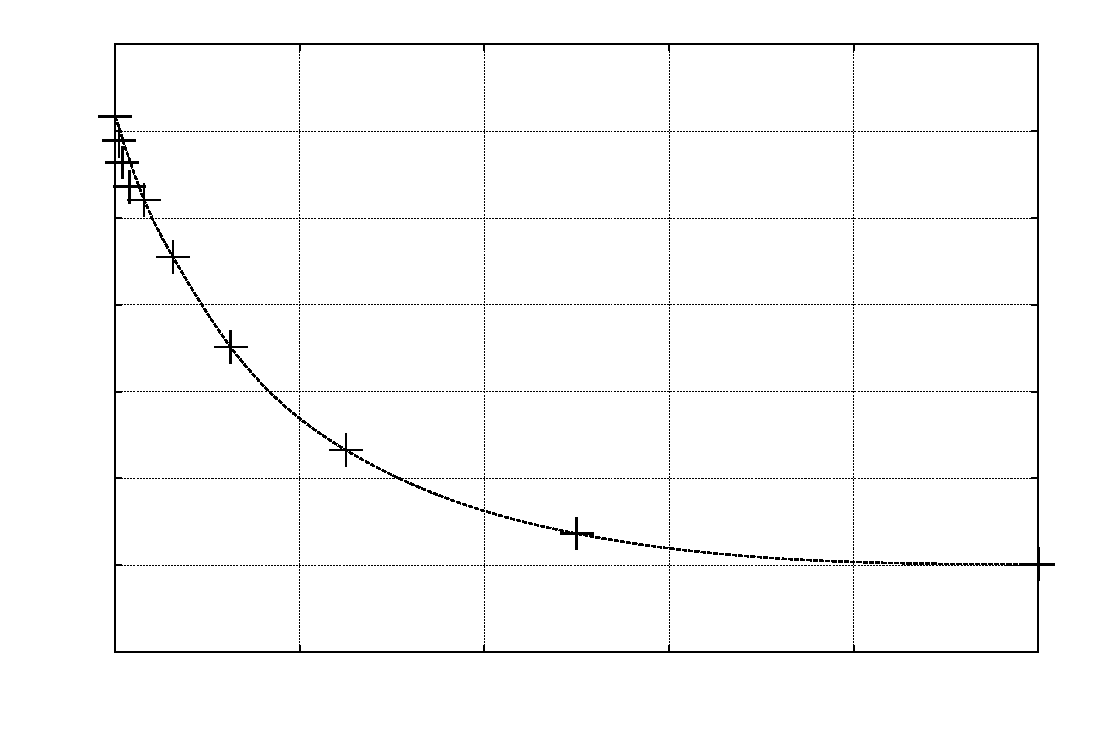
\includegraphics{graf}}%
    \gplfronttext
  \end{picture}%
\endgroup

\caption{Závislost povrchového napětí na koncentraci lihu v roztoku}
\label{grp::graf}
\end{graph}

%Diskuze výsledků
\section*{Diskuze}
Zdroj \cite{napetivoda} uvádí při \SI{20}{\degreeCelsius} povrchové napětí destilované vody (\num{72.75(36)})\,\SI{e-3}{\newton\per\metre} a při \SI{30}{\degreeCelsius} napětí\linebreak (\num{71.99(36)})\,\SI{e-3}{\newton\per\metre}.
Naše hodnota 
\SI{74(3)}{\num{e-3}\,\newton \per \metre}
při \SI{23.5}{\degreeCelsius} se v rámci směrodatné odchylky s těmito hodnotami shoduje.

Zdroj \cite{napetiethanol} uvádí pro teploty okolo \SI{20}{\degreeCelsius} povrchové napětí ethanolu $(\num{22.10} - \num{0.0832}(t- \SI{20}{\degreeCelsius}))$\SI{e-3}{\newton\per\metre}, pro teplotu \SI{23.5}{\degreeCelsius} tedy přibližně \SI{21.8}{\num{e-3}\,\newton \per \metre}.
Naše hodnota \SI{25(2)}{\num{e-3}\,\newton \per \metre} se s ní shoduje v rámci dvou směrodatných odchylek.

Při mísení lihu s vodou dochází k exotermické reakci a směs se zahřívá.
Po smíchání jsme před měřením vždy chvíli počkali, ale směs mohla mít stále nepatrně vyšší teplotu.
Povrchové napětí je na teplotě závislé, chybu způsobenou změnou teploty ale považujeme za menší než chybu způsobenou nepřesností měření, náhodnými jevy a systematickou chybu metody a zanedbáváme ji. 

Další efekt, který mohl způsobit chybu, je kontrakce objemu při mísení lihu s vodou.
Po dvojnásobném zředení v poměru $1:1$ totiž nevznikne roztok o stejné koncentraci jako po jednom zředění v poměru $1:3$.
Tuto chybu však považujeme za zanedbatelnou s ohledem na další nepřesnosti při mísení.

Použitý líh samozřejmě nebyl stoprocentní.
Uvedené koncentrace pouze vyjadřují poměr, ve kterém jsme ho mísili s destilovanou vodou.

%Závěr
\section*{Závěr}
Měřili jsme  závislost povrchového napětí na koncentraci lihu v roztoku.
Změřili jsme povrchové napětí destilované vody (\SI{82(3)}{\num{e-3}\,\si{\newton \per \metre}}) a čistého lihu (\SI{30(2)}{\num{e-3}\,\si{\newton \per \metre}}) při teplotě \SI{23.5(3)}{\degreeCelsius}.
Tyto hodnoty se sice příliš neshodují s tabelovanými, ale obě se od nich liší přibližně o stejnou hodnotu, takže můžeme předpokládat, že naše měření bylo zatíženo stálou systematickou chybou.
To znamená, že se nám sice nepodařilo změřit spolehlivě přímo povrchové napětí, nicméně klesající trend (viz graf \ref{grp::graf}) při zvyšování koncentrace lihu považujeme za velmi správný.
Při nízkých koncentracích má přidání i malého objemu lihu za následek rapidní pokles povrchového napětí, při vyšších koncentracích již efekt není příliš patrný.


\printbibliography[title={Seznam použité literatury}]

\end{document}